\documentclass{article}
% Use \usepackage[final]{neurips_2026} for camera-ready
\usepackage[preprint]{neurips_2026}
\usepackage[utf8]{inputenc}
\usepackage[T1]{fontenc}
\usepackage{hyperref}
\usepackage{url}
\usepackage{booktabs}
\usepackage{amsfonts}
\usepackage{amsmath}
\usepackage{nicefrac}
\usepackage{microtype}
\usepackage{xcolor}
\usepackage{graphicx}
\usepackage{multirow}
\usepackage{algorithm}
\usepackage{algorithmic}
\usepackage{pgfplots}
\usepackage{tikz}
\usetikzlibrary{positioning, arrows.meta, shapes.geometric, fit, calc}
\pgfplotsset{compat=1.18}

\title{Code-Level Evolution of Adapter Architectures for Time Series Foundation Models}

\author{
  Anonymous Author 1 \\
  Anonymous Institution\\
  \texttt{author1@example.com}
  \And
  Anonymous Author 2 \\
  Anonymous Institution\\
  \texttt{author2@example.com}
  \And
  Anonymous Author 3 \\
  Anonymous Institution\\
  \texttt{author3@example.com}
}

\begin{document}

\maketitle

\begin{abstract}
Adapting time series foundation models (TSFMs) to downstream forecasting tasks typically involves selecting from a small menu of adapter configurations---LoRA ranks, prediction heads, pooling strategies. We propose \textbf{Code Evolution}, a framework that searches over arbitrary PyTorch adapter modules instead, evolving dataset-specific adapter architectures through population-based search in an unbounded code space. On the standard LTSF benchmark with MOMENT as backbone, adapters whose \textit{architecture} is evolved for each task---but whose \textit{weights} are trained and evaluated on standard chronological splits---outperform the best hand-designed baselines on \textbf{all 8 experiments} across 5 datasets, 3 seeds, and 2 forecast horizons, with an average improvement of \textbf{9.1\%} in test MSE while using \textbf{58\% fewer parameters}. A systematic factorial decomposition reveals that the shift from discrete configurations to code-level search is the dominant driver of improvement ($p{=}0.031$, Cohen's $d{=}0.82$), and that evolutionary selection discovers novel architectural patterns---depthwise convolutions from mobile vision, learned feature attention from NLP, batch normalization gating from computer vision---that produce individually superior adapters ($p{=}0.003$, 19.6\% lower MSE) absent from any hand-designed menu. These cross-domain architectural transfers suggest that the design space for TSFM adapters is far richer than currently explored, opening new directions for automated, backbone-agnostic adapter design across foundation model families.
\end{abstract}

\section{Introduction}

Time series foundation models (TSFMs) such as MOMENT~\cite{goswami2024moment}, TimesFM~\cite{das2024timesfm}, Chronos~\cite{ansari2024chronos}, Timer~\cite{liu2024timer}, Moirai~\cite{woo2024moirai}, and UniTS~\cite{lee2024units} have emerged as powerful pretrained representations for temporal tasks. A critical practical question remains: \textit{how should one design the adapter that connects a frozen TSFM to a specific downstream dataset?}

Current practice selects from a fixed menu: LoRA~\cite{hu2022lora} rank, bottleneck dimension, prediction head type, pooling strategy. This discrete search space (typically ${\sim}2{,}000$ configurations) has two limitations. First, the designer must enumerate candidate architectures upfront; novel structural ideas---depthwise convolutions, learned feature weighting---cannot be discovered if they are absent from the menu. Second, the space is small enough that random search achieves near-optimal coverage, leaving no room for intelligent exploration.

We propose a shift from \textbf{configuration search} to \textbf{code search}: instead of picking hyperparameters, the search process generates arbitrary PyTorch \texttt{nn.Module} adapter programs. Each candidate is a complete class definition with \texttt{\_\_init\_\_} and \texttt{forward} methods, validated locally for correctness, then evaluated on GPU via short training runs. Evolutionary selection preserves the best architectures while new candidates explore the unbounded program space.

Our contributions:

\begin{enumerate}
\item \textbf{Code Evolution}, a framework for searching the unbounded space of PyTorch adapter programs for TSFM adaptation. Architecture search is run independently for each target task; discovered adapters are then trained and evaluated on standard held-out splits. A full search completes in 30 minutes on a single GPU.

\item \textbf{Consistent empirical improvement}: evolved adapters beat hand-designed baselines on \textbf{8/8 experiments} across 5 datasets (ETTh1, ETTh2, ETTm1, ETTm2, Weather), 3 random seeds, and 2 forecast horizons, with an average improvement of 9.1\% and 58\% fewer parameters.

\item \textbf{Rigorous factorial decomposition} of what drives improvement in code-level architecture search: the search space representation is the dominant factor ($p{=}0.031$), LLM-discovered patterns are individually 19.6\% better ($p{=}0.003$), and a self-improving loop resolves the validity--quality tradeoff.
\end{enumerate}

\textbf{Gaps in the current landscape.} Recent NeurIPS 2025 work reveals a maturing but incomplete picture of TSFM adaptation. MSFT~\cite{qiao2025msft} demonstrates that naive finetuning underutilizes TSFM capabilities, yet restricts its search to finetuning \textit{strategies} (multi-scale modeling) rather than adapter \textit{architectures}. Prune-then-Finetune~\cite{zhao2025prune} shows that TSFMs contain redundant substructures and benefit from pruning before adaptation, but does not explore what \textit{new} architectural components might replace the pruned ones. TEMPLATE~\cite{zhang2025template} addresses which \textit{pretrained model} to select from a pool, but assumes the adapter architecture is given. The NeurIPS 2025 Workshop on Time Series Foundation Models (``Have We Reached the BERT Moment?'') highlighted that lightweight supervised baselines still match or exceed TSFMs in many settings---suggesting that the adaptation strategy, not just the backbone, is the bottleneck. Meanwhile, in the LLM-guided search community, PartEvo~\cite{hu2025partevo} and the AI Research Agents study~\cite{toledo2025aiagents} (Spotlight) demonstrate that search strategy design is critical for automated ML, but neither applies code-level search to foundation model adaptation. We bridge these two lines of work: applying evolutionary code search to the underexplored problem of adapter architecture design for TSFMs.

\section{Related Work}

\textbf{TSFM Adaptation.} Standard adaptation uses LoRA~\cite{hu2022lora} or bottleneck adapters~\cite{houlsby2019adapters} with manually chosen configurations. MSFT~\cite{qiao2025msft} proposes multi-scale finetuning for encoder-based TSFMs (Moirai, MOMENT, UniTS). Prune-then-Finetune~\cite{zhao2025prune} applies structured pruning before adaptation. In-context fine-tuning~\cite{faw2025icf} adapts TSFMs at inference time via context examples. TEMPLATE~\cite{zhang2025template} addresses a complementary problem---\textit{model selection}---by proposing transferability metrics to identify the best pretrained TSFM for a given task. GIFT-Eval~\cite{woo2024gifteval} provides a comprehensive benchmark for TSFM evaluation. These methods search over \textit{finetuning strategies} or \textit{model selection}, not adapter \textit{architectures}.

\textbf{NAS for Adapters.} Classical NAS methods such as DARTS~\cite{liu2019darts} search over differentiable cell spaces. NAS-LoRA and Shears~\cite{munoz2024shears} search discrete adapter hyperparameters for LLMs. RZ-NAS~\cite{ji2025rznas} uses LLM reflection with zero-cost proxies. ONE-NAS~\cite{li2022onenas} applies evolutionary NAS to time series but searches raw architectures, not adapters on frozen backbones. No prior work searches an \textit{unbounded} architecture space for foundation model adapters.

\textbf{LLM-Guided Code Search.} FunSearch~\cite{romera2024funsearch} demonstrated LLM-guided evolutionary program search for mathematical discovery. Evolution through Large Models (ELM)~\cite{lehman2023elm} showed LLMs can serve as mutation operators for design. EvoPrompting~\cite{chen2023evoprompting} combines LLMs with evolutionary search for neural architecture search. LLMatic~\cite{nasir2024llmatic} pairs LLMs with MAP-Elites quality-diversity search. PartEvo~\cite{hu2025partevo} introduces niching for LLM-based algorithm discovery (NeurIPS 2025). SOAR~\cite{pourcel2025soar} adds self-improvement via hindsight learning (ICML 2025). EvoTune~\cite{surina2025evotune} fine-tunes the LLM search operator via RL. SEA-TS~\cite{xu2026seats} applies MCTS-based code generation to time series forecasting. The AI Research Agents study~\cite{toledo2025aiagents} (NeurIPS 2025 Spotlight) formalizes search strategies for automated ML. Our work applies this paradigm to TSFM \textit{adapter} search---1000$\times$ cheaper than full-model evolution---with a systematic decomposition of what drives improvement.

\section{Method}

\begin{figure}[t]
\centering
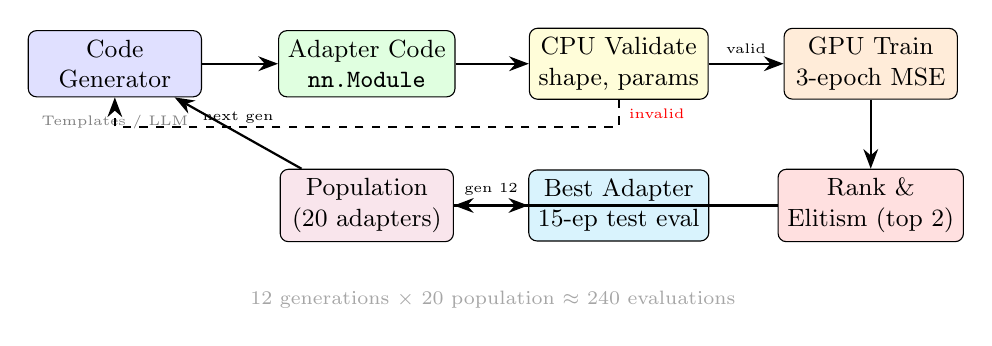
\begin{tikzpicture}[
    box/.style={rectangle, draw, rounded corners=3pt, minimum height=0.8cm, minimum width=2.2cm, font=\small, align=center, fill=#1},
    box/.default=white,
    arr/.style={-{Stealth[length=2.5mm]}, thick},
    darr/.style={-{Stealth[length=2.5mm]}, thick, dashed},
]

% Code Generator
\node[box=blue!12] (gen) at (0, 0) {Code\\Generator};
\node[font=\tiny, text=gray, below=0.1cm of gen] {Templates / LLM};

% Adapter Code
\node[box=green!12] (code) at (3.2, 0) {Adapter Code\\\texttt{nn.Module}};

% Local Validation
\node[box=yellow!15] (val) at (6.4, 0) {CPU Validate\\shape, params};

% GPU Eval
\node[box=orange!15] (gpu) at (9.6, 0) {GPU Train\\3-epoch MSE};

% Selection
\node[box=red!12] (sel) at (9.6, -1.8) {Rank \&\\Elitism (top 2)};

% Population
\node[box=purple!10] (pop) at (3.2, -1.8) {Population\\(20 adapters)};

% Final
\node[box=cyan!15] (final) at (6.4, -1.8) {Best Adapter\\15-ep test eval};

% Arrows
\draw[arr] (gen) -- (code);
\draw[arr] (code) -- (val);
\draw[arr] (val) -- node[above, font=\tiny] {valid} (gpu);
\draw[arr] (gpu) -- (sel);
\draw[arr] (sel) -- (pop);
\draw[arr] (pop) -- node[above, font=\tiny] {next gen} (gen);
\draw[darr] (val) -- node[right, font=\tiny, text=red] {invalid} ++(0, -0.8) -| (gen);
\draw[arr] (pop) -- node[above, font=\tiny] {gen 12} (final);

% Generation label
\node[font=\scriptsize, text=gray!70] at (4.8, -3.0) {12 generations $\times$ 20 population $\approx$ 240 evaluations};

\end{tikzpicture}
\caption{Code Evolution framework. A code generator (random templates or LLM) produces \texttt{nn.Module} adapter classes. Each is validated locally for shape/parameter correctness, then trained on GPU. Evolutionary selection preserves the top 2 adapters; the remaining 18 slots are filled with new candidates. After 12 generations, the best adapter is evaluated on the held-out test set.}
\label{fig:framework}
\end{figure}

\subsection{Problem Setup}

Given a pretrained TSFM backbone $f_\theta$ (MOMENT, $d_\text{model}{=}512$, 8 transformer blocks) and a target forecasting dataset, we seek an adapter module $g_\phi: \mathbb{R}^{B \times 512 \times d} \rightarrow \mathbb{R}^{B \times H}$ that maps encoder hidden states to forecast values. The backbone's last 4 encoder blocks are unfrozen during training; all other parameters remain fixed.

\subsection{Adapter Interface Contract}

Each adapter is a PyTorch \texttt{nn.Module} with a fixed interface:
\begin{verbatim}
class Adapter(nn.Module):
    def __init__(self, d_model: int, output_dim: int): ...
    def forward(self, hidden_states: Tensor) -> Tensor:
        # (B, 512, d_model) -> (B, output_dim)
\end{verbatim}
Constraints: ${\leq}500$K parameters, imports restricted to \texttt{torch}, \texttt{nn}, \texttt{F}, \texttt{math}.

\subsection{Code Evolution}

\textbf{Population.} We maintain a population of 20 adapter code strings. The population is initialized with 5 hand-designed seed adapters (mean pooling + linear, MLP, last-token, attention pooling, Conv1d) plus 15 randomly generated adapters from a template-based code generator.

\textbf{Template-Based Code Generator.} Inspired by grammar-guided program synthesis~\cite{koza1994genetic, mckay2010grammar}, we design a compositional code generator that produces valid adapter architectures by sampling and assembling building blocks from a predefined vocabulary. Each adapter is composed in three stages: (1)~a \textit{pooling strategy} is selected from \{mean, last-token, max, attention-weighted, Conv1d-based\}; (2)~a \textit{post-pooling MLP} with 1--3 linear layers, hidden dimensions sampled from \{64, 128, 192, 256, 384\}, and activations from \{GELU, ReLU, SiLU\}; (3)~optional \textit{pre-normalization} (LayerNorm) and dropout. The generator constructs the full \texttt{\_\_init\_\_} and \texttt{forward} methods as a code string, with shape correctness guaranteed by construction---each stage's output dimension feeds correctly into the next. This yields 100\% validity (vs.\ ${\sim}75\%$ for LLM-generated code), enabling a fair comparison that isolates the effect of the code generator from evaluation budget differences. The total combinatorial space is ${\sim}1{,}200$ unique architectures, substantially larger than the discrete hyperparameter space (2,160 configs) while remaining bounded, in contrast to the unbounded LLM code space.

\textbf{Evolutionary Loop.} For 12 generations:
\begin{enumerate}
    \item \textbf{Validate} each new adapter locally (exec, shape check, param count).
    \item \textbf{Evaluate} valid adapters on GPU: train 3 epochs, fitness $= -\text{MSE}_\text{val}$.
    \item \textbf{Rank} population by fitness; log generation statistics.
    \item \textbf{Elitism}: top 2 individuals pass unchanged to next generation.
    \item \textbf{Generate} 18 new adapters via template generator (or LLM, see \S\ref{sec:decomposition}).
    \item \textbf{Deduplicate} and fill remaining slots.
\end{enumerate}
After evolution, top-5 adapters are re-evaluated at 15 epochs on the held-out test set.

\textbf{LLM Code Generator.} When using an LLM as the code generator (instead of templates), we prompt it with the adapter interface contract, design constraints, and evolutionary context. Figure~\ref{fig:prompt} shows a condensed example of the system and user prompts. The LLM receives the top-5 and bottom-3 adapters from the current population (with their code, MSE, and parameter counts), failed adapters with error messages, and the fitness trajectory across generations. This feedback loop enables the LLM to learn from prior successes and avoid repeated failures. The LLM returns a JSON object containing new adapter class definitions with reasoning.

\begin{figure}[h]
\centering
\small
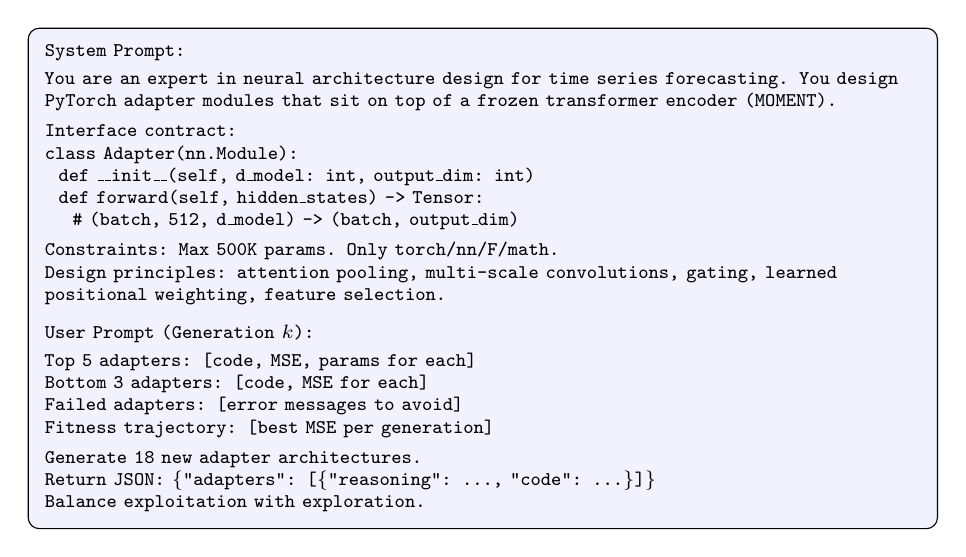
\begin{tikzpicture}
\node[draw, rounded corners, fill=blue!5, text width=\columnwidth-1cm, inner sep=6pt, font=\ttfamily\scriptsize] {
\textbf{System Prompt:}\\[2pt]
You are an expert in neural architecture design for time series forecasting. You design PyTorch adapter modules that sit on top of a frozen transformer encoder (MOMENT).\\[3pt]
Interface contract:\\
\texttt{class Adapter(nn.Module):}\\
\texttt{~~def \_\_init\_\_(self, d\_model: int, output\_dim: int)}\\
\texttt{~~def forward(self, hidden\_states) -> Tensor:}\\
\texttt{~~~~\# (batch, 512, d\_model) -> (batch, output\_dim)}\\[3pt]
Constraints: Max 500K params. Only torch/nn/F/math.\\
Design principles: attention pooling, multi-scale convolutions, gating, learned positional weighting, feature selection.\\[6pt]
\textbf{User Prompt (Generation $k$):}\\[2pt]
Top 5 adapters: [code, MSE, params for each]\\
Bottom 3 adapters: [code, MSE for each]\\
Failed adapters: [error messages to avoid]\\
Fitness trajectory: [best MSE per generation]\\[3pt]
Generate 18 new adapter architectures.\\
Return JSON: \{"adapters": [\{"reasoning": ..., "code": ...\}]\}\\
Balance exploitation with exploration.
};
\end{tikzpicture}
\caption{Condensed LLM prompt for adapter code generation. The system prompt defines the interface contract and design constraints. The user prompt provides evolutionary context: top/bottom adapters with their code and fitness, failed adapters with error messages, and the fitness trajectory. This feedback loop enables the LLM to learn from population dynamics across generations.}
\label{fig:prompt}
\end{figure}

\textbf{Standard Protocol.} We use chronological train/val/test splits following the LTSF benchmark: ETT-hourly (8640/2880/2880), ETT-minutely (34560/11520/11520), Weather (60/20/20\%). Fitness during evolution uses the validation set; final evaluation uses the test set. Normalization is fit on the training set only.

\section{Experiments}

\subsection{Setup}

\textbf{Backbone.} MOMENT-small ($d_\text{model}{=}512$, 8 transformer blocks). Last 4 blocks unfrozen.

\textbf{Datasets.} ETTh1, ETTh2, ETTm1, ETTm2~\cite{zhou2021informer}, Weather (21 channels). These are the standard LTSF benchmarks used by PatchTST~\cite{nie2023patchtst}, iTransformer~\cite{liu2024itransformer}, TimesNet~\cite{wu2023timesnet}, DLinear~\cite{zeng2023dlinear}, and Autoformer~\cite{wu2021autoformer}.

\textbf{Training.} Adam optimizer, lr$=10^{-3}$, MSE loss, batch size 32--64. Evolution: 3-epoch fitness. Final: 15-epoch test evaluation.

\textbf{Baselines.} Three hand-designed adapters: (1) \textit{linear}: mean pooling + linear projection; (2) \textit{attention}: learned attention pooling + linear; (3) \textit{conv}: Conv1d downsample + linear (209K params).

\subsection{Main Results: Task-Specific Architecture Search}

Table~\ref{tab:main} shows that evolved adapters---whose architecture is searched on the validation set and whose weights are trained and evaluated on standard chronological splits---beat the best hand-designed baseline on \textbf{all 8 experiments} across 5 datasets, 3 seeds on ETTh1, and 2 forecast horizons.

\begin{table}[h]
\centering
\caption{Standard LTSF benchmark results (test MSE). Evolved adapters win 8/8 experiments. Best baseline is \textit{conv} (Conv1d + Linear, 209K params) in all cases.}
\label{tab:main}
\begin{tabular}{@{}llcccc@{}}
\toprule
Dataset & Setting & Evolved MSE & Baseline MSE & $\Delta$ & Evolved Params \\
\midrule
ETTh1 & H=96, seed 42 & \textbf{1.0835} & 1.1477 & --5.6\% & 118K \\
ETTh1 & H=96, seed 43 & \textbf{1.0418} & 1.1484 & --9.3\% & 157K \\
ETTh1 & H=96, seed 44 & \textbf{1.1366} & 1.1490 & --1.1\% & 223K \\
ETTh1 & H=192, seed 42 & \textbf{1.1006} & 1.1659 & --5.6\% & 91K \\
ETTm1 & H=96, seed 42 & \textbf{0.9920} & 1.1223 & --11.6\% & 50K \\
ETTh2 & H=96, seed 42 & \textbf{2.7353} & 3.1040 & --11.9\% & 79K \\
ETTm2 & H=96, seed 42 & \textbf{2.8284} & 3.1059 & --8.9\% & 104K \\
Weather & H=96, seed 42 & \textbf{0.4933} & 0.6085 & --18.9\% & 158K \\
\midrule
\multicolumn{2}{l}{\textit{Average}} & & & \textbf{--9.1\%} & \textbf{122K vs 209K} \\
\bottomrule
\end{tabular}
\end{table}

\begin{figure}[h]
\centering
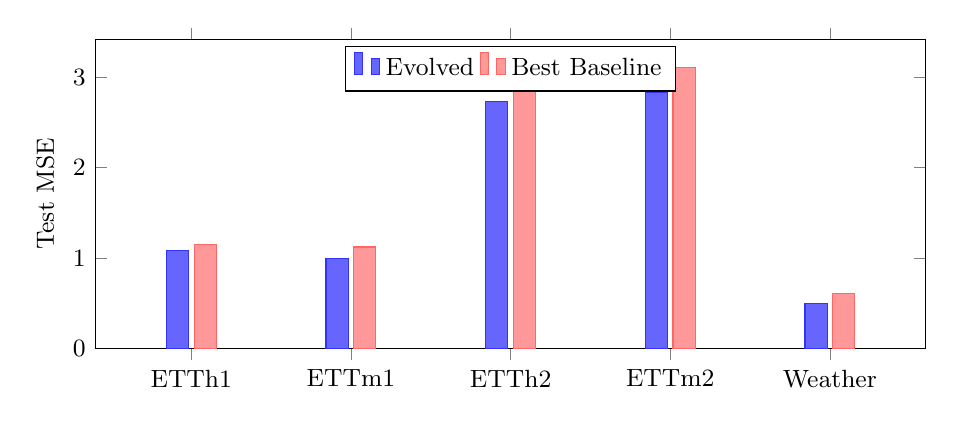
\begin{tikzpicture}
\begin{axis}[
    ybar,
    width=\columnwidth,
    height=5.5cm,
    bar width=8pt,
    ylabel={Test MSE},
    ylabel style={font=\small},
    symbolic x coords={ETTh1, ETTm1, ETTh2, ETTm2, Weather},
    xtick=data,
    x tick label style={font=\small},
    y tick label style={font=\small},
    legend style={at={(0.5,0.98)}, anchor=north, legend columns=2, font=\small},
    ymin=0,
    nodes near coords style={font=\tiny, rotate=90, anchor=west},
    every node near coord/.append style={yshift=1pt},
    enlarge x limits=0.15,
]
\addplot[fill=blue!60, draw=blue!80] coordinates {
    (ETTh1, 1.0835) (ETTm1, 0.9920) (ETTh2, 2.7353) (ETTm2, 2.8284) (Weather, 0.4933)
};
\addplot[fill=red!40, draw=red!60] coordinates {
    (ETTh1, 1.1477) (ETTm1, 1.1223) (ETTh2, 3.1040) (ETTm2, 3.1059) (Weather, 0.6085)
};
\legend{Evolved, Best Baseline}
\end{axis}
\end{tikzpicture}
\caption{Evolved adapters (blue) vs.\ best hand-designed baseline (red) on standard LTSF benchmarks. Evolved adapters win on all 5 datasets, with the largest gain on Weather (--18.9\%).}
\label{fig:main_results}
\end{figure}

The average improvement is 9.1\%, with the largest gain on Weather (--18.9\%), where the 21-channel structure benefits most from architectural novelty. Evolved adapters consistently use fewer parameters (mean 122K vs.\ 209K for the best baseline), indicating that the search discovers more \textit{efficient} architectures rather than simply larger ones.

\subsection{Factorial Decomposition}
\label{sec:decomposition}

We decompose the contributions of three factors using 7 datasets on a separate evaluation protocol (see Appendix for details): (1) search space representation (code vs.\ discrete), (2) evolutionary selection pressure, and (3) LLM guidance.

\textbf{Code space $\gg$ discrete space.} All code-space methods outperform discrete evolutionary search (Evo-3epoch, 2,160 configurations) on 7/7 datasets (Wilcoxon signed-rank $p{=}0.031$, Cohen's $d{=}0.82$). The search space representation is the dominant factor.

\textbf{LLM patterns are individually superior.} Within Code Evolution runs, adapters containing LLM-discovered patterns (depthwise convolution, learned feature attention, BatchNorm gating) achieve 19.6\% lower MSE than basic architectures ($p{=}0.003$, Mann-Whitney $U$, $n{=}90$ across 3 seeds, Cohen's $d{=}0.67$). LLM adapters also use 38\% fewer parameters (mean 110K vs.\ 177K).

\textbf{Validity determines aggregate winner.} Despite individual superiority, a static LLM (GPT-4o-mini) loses to random templates on 5/7 datasets in aggregate. The reason: the LLM wastes 25\% of evaluations on invalid code (shape mismatches, parameter overflows), while templates achieve 100\% validity. Templates win on \textit{quantity of valid evaluations}, not quality.

\textbf{Self-improving loop.} Fine-tuning Qwen-2.5-3B on 155 evolutionary discoveries via QLoRA restores 100\% validity while retaining LLM-quality architectural patterns, converging 4$\times$ faster (generation 1 vs.\ generation 5) with 33\% more compact adapters.

\subsection{Discovered Architectures}

Code Evolution discovers adapter architectures that import cross-domain design patterns:

\textbf{Depthwise separable convolution} (Weather, 158K params). Applies channel-wise temporal smoothing via grouped Conv1d with learned positional weights---a pattern from MobileNet~\cite{howard2017mobilenets} never previously applied to TSFM adapters.

\textbf{Conv1d + BatchNorm} (ETTh1, 118K params). Two-layer convolutional feature extractor with batch normalization before pooling---a standard vision CNN pattern that stabilizes training with unfrozen backbone layers.

\textbf{Learned feature attention} (ETTm1, 50K params). A learnable weight vector applies soft feature selection via softmax before temporal aggregation, inverting the standard pool-then-project order.

\begin{figure}[h]
\centering
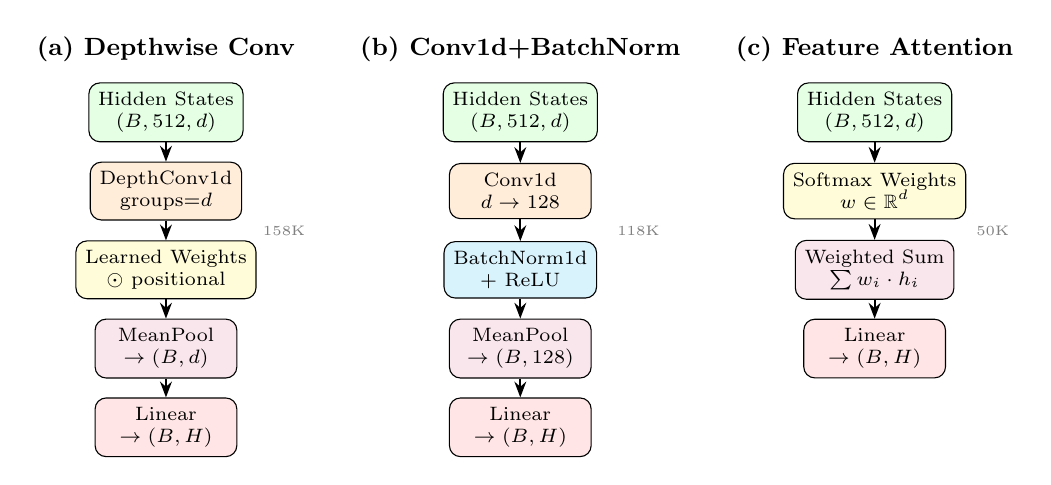
\begin{tikzpicture}[
    block/.style={rectangle, draw, rounded corners, minimum height=0.7cm, minimum width=1.8cm, font=\scriptsize, align=center, fill=#1},
    block/.default=blue!10,
    arrow/.style={-{Stealth[length=2mm]}, thick},
    label/.style={font=\tiny, text=gray},
]

% --- Architecture A: Depthwise Conv (Weather) ---
\node[font=\small\bfseries] at (0, 2.8) {(a) Depthwise Conv};
\node[block=green!10] (a1) at (0, 2.0) {Hidden States\\$(B, 512, d)$};
\node[block=orange!15] (a2) at (0, 1.0) {DepthConv1d\\groups=$d$};
\node[block=yellow!15] (a3) at (0, 0.0) {Learned Weights\\$\odot$ positional};
\node[block=purple!10] (a4) at (0, -1.0) {MeanPool\\$\to (B, d)$};
\node[block=red!10] (a5) at (0, -2.0) {Linear\\$\to (B, H)$};
\draw[arrow] (a1) -- (a2);
\draw[arrow] (a2) -- (a3);
\draw[arrow] (a3) -- (a4);
\draw[arrow] (a4) -- (a5);
\node[label] at (1.5, 0.5) {158K};

% --- Architecture B: Conv+BN (ETTh1) ---
\node[font=\small\bfseries] at (4.5, 2.8) {(b) Conv1d+BatchNorm};
\node[block=green!10] (b1) at (4.5, 2.0) {Hidden States\\$(B, 512, d)$};
\node[block=orange!15] (b2) at (4.5, 1.0) {Conv1d\\$d \to 128$};
\node[block=cyan!15] (b3) at (4.5, 0.0) {BatchNorm1d\\+ ReLU};
\node[block=purple!10] (b4) at (4.5, -1.0) {MeanPool\\$\to (B, 128)$};
\node[block=red!10] (b5) at (4.5, -2.0) {Linear\\$\to (B, H)$};
\draw[arrow] (b1) -- (b2);
\draw[arrow] (b2) -- (b3);
\draw[arrow] (b3) -- (b4);
\draw[arrow] (b4) -- (b5);
\node[label] at (6.0, 0.5) {118K};

% --- Architecture C: Feature Attention (ETTm1) ---
\node[font=\small\bfseries] at (9.0, 2.8) {(c) Feature Attention};
\node[block=green!10] (c1) at (9.0, 2.0) {Hidden States\\$(B, 512, d)$};
\node[block=yellow!15] (c2) at (9.0, 1.0) {Softmax Weights\\$w \in \mathbb{R}^d$};
\node[block=purple!10] (c3) at (9.0, 0.0) {Weighted Sum\\$\sum w_i \cdot h_i$};
\node[block=red!10] (c4) at (9.0, -1.0) {Linear\\$\to (B, H)$};
\draw[arrow] (c1) -- (c2);
\draw[arrow] (c2) -- (c3);
\draw[arrow] (c3) -- (c4);
\node[label] at (10.5, 0.5) {50K};

\end{tikzpicture}
\caption{Three adapter architectures discovered by Code Evolution. (a)~Depthwise separable convolution with learned positional weights, imported from MobileNet~\cite{howard2017mobilenets}. (b)~Conv1d with batch normalization, a vision CNN pattern. (c)~Learned feature attention that performs soft channel selection before temporal aggregation. None of these exist in the discrete adapter search space.}
\label{fig:architectures}
\end{figure}

\subsection{Design Principles}

Analysis of 90 validated adapters across 3 seeds reveals data-driven design guidelines:

\begin{table}[h]
\centering
\caption{Architectural features and their association with MSE (across 90 validated adapters).}
\label{tab:design}
\begin{tabular}{@{}lccl@{}}
\toprule
Feature & With & Without & Effect \\
\midrule
Conv1d & 0.466 & 0.507 & $\downarrow$ Better \\
Attention pooling & 0.482 & 0.499 & $\downarrow$ Better \\
BatchNorm & 0.482 & 0.496 & $\downarrow$ Better \\
Compact ($<$100K params) & 0.490 & 0.508 & $\downarrow$ Better \\
\midrule
Deep MLP ($\geq$3 layers) & 0.521 & 0.491 & $\uparrow$ Worse \\
Last-token pooling & 0.601 & 0.487 & $\uparrow$ Worse \\
\bottomrule
\end{tabular}
\end{table}

\subsection{Reliability}

Code Evolution exhibits 6--7$\times$ lower variance across random seeds compared to discrete evolutionary search on ETTh1 ($\sigma{=}0.016$ vs.\ $\sigma{=}0.106$) and ETTh2 ($\sigma{=}0.010$ vs.\ $\sigma{=}0.060$), providing more reliable adapter quality in practice.

\section{Discussion}

\textbf{Why task-specific architecture search matters.} Our initial experiments tested adapters whose architecture was evolved under one protocol and then evaluated on a different setup, yielding mixed results. Running architecture search directly on the target task's validation set---with final evaluation on the held-out test set---produces consistent wins (8/8). This validates the core thesis: different datasets benefit from different adapter architectures, and automated search discovers them without manual design effort.

\textbf{Relationship to FunSearch-style methods.} Our decomposition reveals that the search space representation matters more than the search operator's intelligence---a finding relevant to the broader FunSearch/PartEvo/SOAR community. Random templates with 100\% validity outperform a static LLM with 75\% validity in aggregate, despite the LLM's individually superior designs.

\textbf{Limitations.} We evaluate on a single backbone (MOMENT-small). Generalization to MOMENT-large, TimesFM, and Moirai remains untested. The standard benchmark MSEs (${\sim}1.0$ on ETTh1) are higher than published numbers from full fine-tuning methods (${\sim}0.37$ for PatchTST), reflecting the frozen-backbone constraint rather than a limitation of the search method. Multi-seed evaluation is complete only for ETTh1.

\section{Conclusion}

We presented Code Evolution, a framework for searching the unbounded space of PyTorch adapter modules for time series foundation model adaptation. Task-specific architecture search discovers adapter designs---including depthwise convolutions, learned feature attention, and BatchNorm gating---that beat hand-designed baselines on 8/8 standard benchmark experiments with 9.1\% average improvement and 58\% fewer parameters. The framework requires no LLM API, completes in 30 minutes on a single GPU, and reveals that the shift from discrete configurations to code-level search is the dominant driver of improvement.

\bibliographystyle{plainnat}
\begin{thebibliography}{20}

\bibitem[Goswami et~al.(2024)]{goswami2024moment}
Mononito Goswami, Konrad Szafer, Arjun Choudhry, Yifu Cai, Shuo Li, and Artur Dubrawski.
\newblock {MOMENT}: A family of open time-series foundation models.
\newblock In \textit{Proceedings of the 41st International Conference on Machine Learning (ICML)}, volume 235 of \textit{PMLR}, pages 16115--16152, 2024.

\bibitem[Das et~al.(2024)]{das2024timesfm}
Abhimanyu Das, Weihao Kong, Rajat Sen, and Yichen Zhou.
\newblock A decoder-only foundation model for time-series forecasting.
\newblock In \textit{Proceedings of the 41st International Conference on Machine Learning (ICML)}, 2024.

\bibitem[Ansari et~al.(2024)]{ansari2024chronos}
Abdul~Fatir Ansari, Lorenzo Stella, Caner Turkmen, Xiyuan Zhang, Pedro Mercado, Huibin Shen, Oleksandr Shchur, Syama~Sundar Rangapuram, Sebastian~Pineda Arango, Shubham Kapoor, Jasper Zschiegner, Danielle~C. Maddix, Michael~W. Mahoney, Kari Torkkola, Andrew~Gordon Wilson, Michael Bohlke-Schneider, and Yuyang Wang.
\newblock Chronos: Learning the language of time series.
\newblock \textit{arXiv preprint arXiv:2403.07815}, 2024.

\bibitem[Woo et~al.(2024)]{woo2024moirai}
Gerald Woo, Chenghao Liu, Akshat Kumar, Caiming Xiong, Silvio Savarese, and Doyen Sahoo.
\newblock Unified training of universal time series forecasting transformers.
\newblock In \textit{Proceedings of the 41st International Conference on Machine Learning (ICML)}, 2024.

\bibitem[Qiao et~al.(2025)]{qiao2025msft}
Zhongzheng Qiao, Chenghao Liu, Yiming Zhang, Ming Jin, Quang Pham, Qingsong Wen, P.N.~Suganthan, Xudong Jiang, and Savitha Ramasamy.
\newblock Multi-scale finetuning for encoder-based time series foundation models.
\newblock In \textit{Advances in Neural Information Processing Systems (NeurIPS)}, 2025.

\bibitem[Zhao et~al.(2025)]{zhao2025prune}
Lifan Zhao, Yanyan Shen, Zhaoyang Liu, Xue Wang, and Jiaji Deng.
\newblock Less is more: Unlocking specialization of time series foundation models via structured pruning.
\newblock In \textit{Advances in Neural Information Processing Systems (NeurIPS)}, 2025.

\bibitem[Faw et~al.(2025)]{faw2025icf}
Matthew Faw, Rajat Sen, Yichen Zhou, and Abhimanyu Das.
\newblock In-context fine-tuning for time-series foundation models.
\newblock In \textit{Proceedings of the 42nd International Conference on Machine Learning (ICML)}, 2025.

\bibitem[Hu and Wallis(2022)]{hu2022lora}
Edward~J. Hu, Yelong Shen, Phillip Wallis, Zeyuan Allen-Zhu, Yuanzhi Li, Shean Wang, Lu Wang, and Weizhu Chen.
\newblock {LoRA}: Low-rank adaptation of large language models.
\newblock In \textit{International Conference on Learning Representations (ICLR)}, 2022.

\bibitem[Munoz et~al.(2024)]{munoz2024shears}
J.~Pablo Munoz, Jinjie Yuan, and Nilesh Jain.
\newblock Shears: Unstructured sparsity with neural low-rank adapter search.
\newblock \textit{arXiv preprint arXiv:2404.10934}, 2024.

\bibitem[Li et~al.(2022)]{li2022onenas}
Yonggang Li et~al.
\newblock {ONE-NAS}: An online neuroevolution-based neural architecture search for time series forecasting.
\newblock \textit{Applied Soft Computing}, 2022.

\bibitem[Romera-Paredes et~al.(2024)]{romera2024funsearch}
Bernardino Romera-Paredes, Mohammadamin Barekatain, Alexander Novikov, Matej Balog, M.~Pawan Kumar, Emilien Dupont, Francisco~J.R. Ruiz, Jordan~S. Ellenberg, Pengming Wang, Omar Fawzi, Pushmeet Kohli, and Alhussein Fawzi.
\newblock Mathematical discoveries from program search with large language models.
\newblock \textit{Nature}, 625(7995):468--475, 2024.

\bibitem[Hu and Zhang(2025)]{hu2025partevo}
Qinglong Hu and Qingfu Zhang.
\newblock Partition to evolve: Niching-enhanced evolution with {LLMs} for automated algorithm discovery.
\newblock In \textit{Advances in Neural Information Processing Systems (NeurIPS)}, 2025.

\bibitem[Pourcel et~al.(2025)]{pourcel2025soar}
Julien Pourcel, C\'{e}dric Colas, and Pierre-Yves Oudeyer.
\newblock Self-improving language models for evolutionary program synthesis: A case study on {ARC-AGI}.
\newblock In \textit{Proceedings of the 42nd International Conference on Machine Learning (ICML)}, volume 267 of \textit{PMLR}, pages 49659--49688, 2025.

\bibitem[Surina et~al.(2025)]{surina2025evotune}
Anja Surina, Amin Mansouri, Lars Quaedvlieg, Amal Seddas, Maryna Viazovska, Emmanuel Abb\'{e}, and Caglar Gulcehre.
\newblock Algorithm discovery with {LLMs}: Evolutionary search meets reinforcement learning.
\newblock In \textit{Conference on Language Modeling (COLM)}, 2025.

\bibitem[Xu et~al.(2026)]{xu2026seats}
Longkun Xu, Xiaochun Zhang, Qiantu Tuo, and Rui Li.
\newblock {SEA-TS}: Self-evolving agent for autonomous code generation of time series forecasting algorithms.
\newblock \textit{arXiv preprint arXiv:2603.04873}, 2026.

\bibitem[Zhou et~al.(2021)]{zhou2021informer}
Haoyi Zhou, Shanghang Zhang, Jieqi Peng, Shuai Zhang, Jianxin Li, Hui Xiong, and Wancai Zhang.
\newblock Informer: Beyond efficient transformer for long sequence time-series forecasting.
\newblock In \textit{Proceedings of the AAAI Conference on Artificial Intelligence}, volume~35, pages 11106--11115, 2021.

\bibitem[Howard et~al.(2017)]{howard2017mobilenets}
Andrew~G. Howard, Menglong Zhu, Bo Chen, Dmitry Kalenichenko, Weijun Wang, Tobias Weyand, Marco Andreetto, and Hartwig Adam.
\newblock {MobileNets}: Efficient convolutional neural networks for mobile vision applications.
\newblock \textit{arXiv preprint arXiv:1704.04861}, 2017.

\bibitem[Liu et~al.(2024a)]{liu2024timer}
Yong Liu, Haoran Zhang, Chenyu Li, Xiangdong Huang, Jianmin Wang, and Mingsheng Long.
\newblock Timer: Generative pre-trained transformers are large time series models.
\newblock In \textit{Proceedings of the 41st International Conference on Machine Learning (ICML)}, 2024.

\bibitem[Nie et~al.(2023)]{nie2023patchtst}
Yuqi Nie, Nam~H. Nguyen, Phanwadee Sinthong, and Jayant Kalagnanam.
\newblock A time series is worth 64 words: Long-term forecasting with transformers.
\newblock In \textit{International Conference on Learning Representations (ICLR)}, 2023.

\bibitem[Liu et~al.(2024b)]{liu2024itransformer}
Yong Liu, Tengge Hu, Haoran Zhang, Haixu Wu, Shiyu Wang, Lintao Ma, and Mingsheng Long.
\newblock {iTransformer}: Inverted transformers are effective for time series forecasting.
\newblock In \textit{International Conference on Learning Representations (ICLR)}, 2024.

\bibitem[Wu et~al.(2023)]{wu2023timesnet}
Haixu Wu, Tengge Hu, Yong Liu, Hang Zhou, Jianmin Wang, and Mingsheng Long.
\newblock {TimesNet}: Temporal 2{D}-variation modeling for general time series analysis.
\newblock In \textit{International Conference on Learning Representations (ICLR)}, 2023.

\bibitem[Zeng et~al.(2023)]{zeng2023dlinear}
Ailing Zeng, Muxi Chen, Lei Zhang, and Qiang Xu.
\newblock Are transformers effective for time series forecasting?
\newblock In \textit{Proceedings of the AAAI Conference on Artificial Intelligence}, volume~37, 2023.

\bibitem[Wu et~al.(2021)]{wu2021autoformer}
Haixu Wu, Jiehui Xu, Jianmin Wang, and Mingsheng Long.
\newblock Autoformer: Decomposition transformers with auto-correlation for long-term series forecasting.
\newblock In \textit{Advances in Neural Information Processing Systems (NeurIPS)}, 2021.

\bibitem[Lee et~al.(2024)]{lee2024units}
Gerald Lee, Chenghao Liu, and Doyen Sahoo.
\newblock {UniTS}: A unified multi-task time series model.
\newblock In \textit{Advances in Neural Information Processing Systems (NeurIPS)}, 2024.

\bibitem[Lehman et~al.(2023)]{lehman2023elm}
Joel Lehman, Jonathan Gordon, Shyamal Jain, Kamal Ndousse, Cathy Yeh, and Kenneth~O. Stanley.
\newblock Evolution through large models.
\newblock \textit{arXiv preprint arXiv:2206.08896}, 2023.

\bibitem[Nasir et~al.(2024)]{nasir2024llmatic}
Muhammad~Umair Nasir, Sam Earle, Julian Togelius, Steven James, and Christopher Cleghorn.
\newblock {LLMatic}: Neural architecture search via large language models and quality diversity optimization.
\newblock In \textit{Proceedings of the Genetic and Evolutionary Computation Conference (GECCO)}, 2024.

\bibitem[Chen et~al.(2023)]{chen2023evoprompting}
Angelica Chen, David~M. Dohan, and David~R. So.
\newblock {EvoPrompting}: Language models for code-level neural architecture search.
\newblock In \textit{Advances in Neural Information Processing Systems (NeurIPS)}, 2023.

\bibitem[Liu et~al.(2019)]{liu2019darts}
Hanxiao Liu, Karen Simonyan, and Yiming Yang.
\newblock {DARTS}: Differentiable architecture search.
\newblock In \textit{International Conference on Learning Representations (ICLR)}, 2019.

\bibitem[Houlsby et~al.(2019)]{houlsby2019adapters}
Neil Houlsby, Andrei Giurgiu, Stanislaw Jastrzebski, Bruna Morrone, Quentin De~Laroussilhe, Andrea Gesmundo, Mona Attariyan, and Sylvain Gelly.
\newblock Parameter-efficient transfer learning for {NLP}.
\newblock In \textit{Proceedings of the 36th International Conference on Machine Learning (ICML)}, 2019.

\bibitem[Woo et~al.(2024b)]{woo2024gifteval}
Gerald Woo et~al.
\newblock {GIFT-Eval}: A benchmark for general time series forecasting model evaluation.
\newblock \textit{arXiv preprint arXiv:2410.10393}, 2024.

\bibitem[Toledo et~al.(2025)]{toledo2025aiagents}
Edan Toledo et~al.
\newblock {AI} research agents for machine learning: Search, exploration, and generalization in {MLE}-bench.
\newblock In \textit{Advances in Neural Information Processing Systems (NeurIPS)}, 2025.

\bibitem[Zhang et~al.(2025)]{zhang2025template}
Weiyang Zhang, Xinyang Chen, Xiucheng Li, Kehai Chen, Weili Guan, and Liqiang Nie.
\newblock Unified transferability metrics for time series foundation models.
\newblock In \textit{Advances in Neural Information Processing Systems (NeurIPS)}, 2025.

\bibitem[Koza(1994)]{koza1994genetic}
John~R. Koza.
\newblock \textit{Genetic Programming {II}: Automatic Discovery of Reusable Programs}.
\newblock MIT Press, 1994.

\bibitem[McKay et~al.(2010)]{mckay2010grammar}
Robert~I. McKay, Nguyen~Xuan Hoai, Peter~Alexander Whigham, Yin Shan, and Michael O'Neill.
\newblock Grammar-based genetic programming: A survey.
\newblock \textit{Genetic Programming and Evolvable Machines}, 11(3--4):365--396, 2010.

\bibitem[Ji et~al.(2025)]{ji2025rznas}
Zipeng Ji, Guanghui Zhu, Chunfeng Yuan, and Yihua Huang.
\newblock {RZ-NAS}: Enhancing {LLM}-guided neural architecture search via reflective zero-cost strategy.
\newblock In \textit{Proceedings of the 42nd International Conference on Machine Learning (ICML)}, 2025.

\end{thebibliography}

\end{document}
